\chapter{Conclusions and Contributions}\label{ch:conclusion}

\section{Conclusions}
This dissertation developed a coupled thermodynamic, transport, and material-design framework for enhancing thermoelectric performance under transient heating. Across all analyses, the scaffold is explicitly \textbf{polyvinyl alcohol (PVA)} as the continuous matrix; CuS--MoS$_2$ acts as reinforcing nanofillers dispersed within PVA; and PCM is embedded within hierarchical PVA pores.

The findings show that transient thermal buffering from embedded PCM can stabilize interface temperatures and increase cycle-averaged useful gradients. Moderate CuS--MoS$_2$ loading can improve electrical and thermal transport balance, whereas excessive loading degrades interfacial performance. Exergy-based optimization confirms that entropy generation reduction is critical for sustained gains.

\section{Primary Contributions}
\begin{enumerate}
    \item A defense-level unified model coupling Seebeck--Peltier--Thomson transport with latent heat dynamics and porous composite effects.
    \item A clear role-separated material architecture: PVA scaffold, PCM latent storage, CuS--MoS$_2$ reinforcement.
    \item Dimensionless and sensitivity tools to identify robust operating windows under pulsed heat loads.
    \item Entropy and exergy analyses translating multiphysics responses into actionable design criteria.
    \item A validation protocol integrating DSC, SEM, and thermal/electrical metrology with uncertainty propagation.
\end{enumerate}

\section{Final Remarks}
The proposed architecture can be further strengthened by moisture-management strategies, large-area manufacturing controls, and long-duration reliability studies. Nonetheless, the present work establishes a comprehensive foundation for engineering PVA-based PCM-buffered thermoelectric systems with reinforced nanostructural pathways.


\begin{figure}[htbp]
\centering
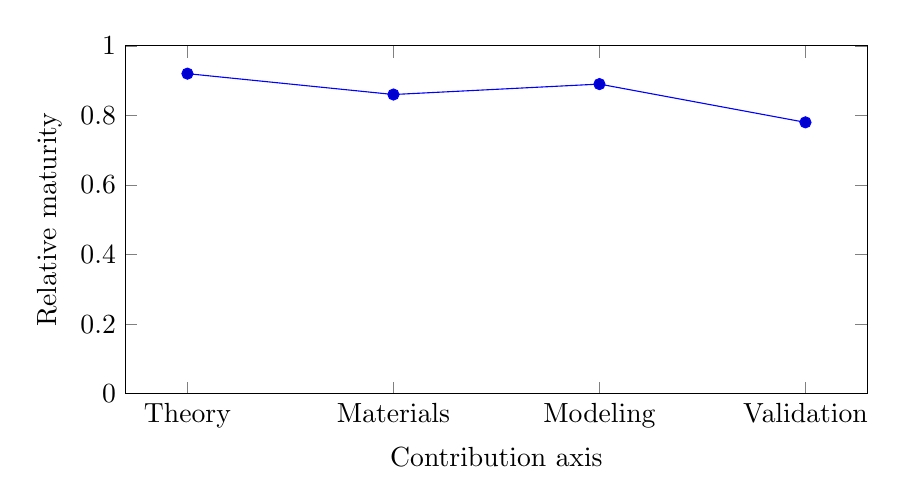
\begin{tikzpicture}
\begin{axis}[width=11cm,height=6cm,xlabel={Contribution axis},ylabel={Relative maturity},symbolic x coords={Theory,Materials,Modeling,Validation},xtick=data,ymin=0,ymax=1]
\addplot+[mark=*] coordinates {(Theory,0.92)(Materials,0.86)(Modeling,0.89)(Validation,0.78)};
\end{axis}
\end{tikzpicture}
\caption{Summary map of contribution maturity across dissertation pillars.}
\label{fig:contrib_map}
\end{figure}
